\documentclass{article}
\usepackage{homework-preamble}

\begin{document}
\title{Honours Analysis: Homework 7}
\author{Franz Miltz (UUN: S1971811)}
\date{11 November 2021}
\maketitle

\section*{Workshop 7 - Question 4}

\begin{claim*}
	Let $I$ be a bounded interval and let $f:I\to\R$ be such that
	\begin{align*}
		f(x) = \begin{cases}
			       1, & \text{for }x\not\in\Q, \\
			       0, & \text{for }x\in\Q.
		       \end{cases}
	\end{align*}
	Then $f$ is integrable and $\int_I f = \lambda(I)$.
\end{claim*}
\begin{proof}
	We can write $f$ as a difference of characteristic functions:
	\begin{align*}
		f(x) = \chi_I(x) - \chi_\Q(x)\hs\text{for all }x\in I.
	\end{align*}
	Note that $\chi_I$ is integrable by definition and $\chi_\Q$ is integrable due to
	\emph{Notes, Exercise 4.4}.

	Thus, by \emph{Notes, Theorem 4.2}, $f$ is integrable and
	\begin{align*}
		\int_I f = \int_I \chi_I - \int_I \chi_\Q = \lambda(I)-0 = \lambda(I).
	\end{align*}
\end{proof}

\section*{Workshop 7 - Question 5}

Let $f:[a,b]\to\R$ be continuous and let $M=\sup_{x\in[a,b]}\abs{f(x)}$. Suppose
$M>0$. Let $p>0$.

\begin{claim*}
	For every $\e$ such that $0<\e<M/2$ there is a non-empty open interval $I\subseteq[a,b]$
	such that
	\begin{align}
		\label{fullineq}
		(M-\e)^p\lambda(I)\leq \int_a^b \abs{f(x)}^p dx \leq M^p(b-a).
	\end{align}
\end{claim*}
\begin{proof}
	Observe that the absolute value function is continuous. Therefore $\abs{f(x)}$
	is a composition of continuous functions and thereby continuous itself.
	By the \emph{Extreme Value Theorem}, there exists $x_0\in[a,b]$ such that
	\begin{align*}
		\abs{f(x_0)} = M.
	\end{align*}
	Further, by continuity of $\abs{f}$, there exists $\delta>0$ such that for all
	$x\in I=(x_0-\delta, x_0+\delta)\cap[a,b]$,
	\begin{align*}
		M-\e < \abs{f(x)}.
	\end{align*}
	Note that $\epsilon > M/2 > 0$ and $p>0$. Therefore
	\begin{align*}
		(M-\e)^p < \abs{f(x)}^p.
	\end{align*}
	By \emph{Notes, Theorem 4.2} we find
	\begin{align*}
		\int_I (M-\e)^p \leq \int_I \abs{f(x)}^pdx.
	\end{align*}
	Since $(M-\e)^p$ is constant and $\abs{f(x)}^p$ is non-negative, we can use
	\emph{Notes, Theorem 4.8} and $I\subset [a,b]$ to write
	\begin{align}
		\label{leftineq}
		(M-\e)^p \lambda(I)=
		\int_I (M-\e)^p \leq \int_I \abs{f(x)}^pdx
		\leq \int_a^b \abs{f(x)}^p dx.
	\end{align}
	Further, we have
	\begin{align*}
		\abs{f(x)}^p \leq M^p
	\end{align*}
	and thus
	\begin{align}
		\label{rightineq}
		\int_a^b \abs{f(x)}^p \leq \int_a^b M^p = M^p(b-a).
	\end{align}
	Combining (\ref{leftineq}) and (\ref{rightineq}), the claim follows.
\end{proof}

\begin{claim*}
	\begin{align*}
		\lim_{p\to\infty} \left(\int_a^b \abs{f(x)}^p dx\right)^{1/p} = M.
	\end{align*}
\end{claim*}
\begin{proof}
	Consider a sequence $(p_n)$ where $p_n>0$ for all $n\in\N$ and
	$p_n\to\infty$ as $n\to\infty$. Then define the sequence $(s_n)$ by
	\begin{align*}
		s_n = \int_a^b \abs{f(x)}^pdx.
	\end{align*}
	Fix $0<\e<M/2$. Then, by (\ref{fullineq}), we have
	\begin{align*}
		(M-\e)^p\lambda(I) \leq s_n \leq M^p(b-a).
	\end{align*}
	where $I\subseteq [a,b]$. Since all the terms are positive, we have
	\begin{align*}
		(M-\e)\left(\lambda(I)\right)^{1/p} \leq
		s_n^{1/p} \leq
		M(b-a)^{1/p}.
	\end{align*}
	Consider the limits
	\begin{align*}
		\lim_{p\to\infty} (M-\e)(\lambda(I))^{1/p} & = M-\e, \\
		\lim_{p\to\infty} M(b-a)^{1/p}             & = M,    \\
	\end{align*}
	Therefore, for any $0<\e<M/2$,
	\begin{align*}
		M-\e \leq \lim_{p\to\infty} s_n^{1/p} \leq M.
	\end{align*}
	Note that $s_n$ does not depend on $\e$ so we must have

	\begin{align*}
		\lim_{p\to\infty} s_n^{1/p} = \lim_{p\to\infty} \left(\int_a^b \abs{f(x)}dx\right)^{1/p} = M.
	\end{align*}
\end{proof}

\subsection*{Workshop 7 - Question 6}

\begin{claim*}
	Let $f(x)=n$ for every $x\in((n+1)^{-2}, n^{-2}]$, $n\in\N$. $f$ is integrable on $(0,1]$
	and
	\begin{align*}
		\int_{(0, 1]} f = \sum_{j=1}^\infty \frac{1}{j^2}.
	\end{align*}
\end{claim*}
\begin{proof}
	Consider the function $g:(0,1]\to\R$ given by
	\begin{align*}
		g(x) = \sum_{j=1}^\infty \chi_{J_j}(x)
	\end{align*}
	where $J_j = (0, j^{-2}]$. Note that for $x\in((n+1)^{-2}, n^{-2}]$ where $n\in\N$,
	we have $\chi_{J_j}(x)=1$ if and only if $j\leq n$. Thus
	\begin{align*}
		g(x) = \sum_{j=1}^n 1 = n = f(x)
	\end{align*}
	for all $x\in(0,1]$. We observe that
	\begin{align*}
		\sum_{j=1}^\infty \abs{c_j} \lambda(J_j) = \sum_{j=1}^\infty \frac{1}{j^2}
	\end{align*}
	with $c_j=1$ which is a converging $p$-series. By definition of Lebesgue integrability,
	we have
	\begin{align*}
		\int_{(0,1]} f = \sum_{j=1}^\infty \lambda(J_j) = \sum_{j=1}^\infty \frac{1}{j^2}.
	\end{align*}
\end{proof}

\paragraph{Sketch of $f$}

\begin{center}
	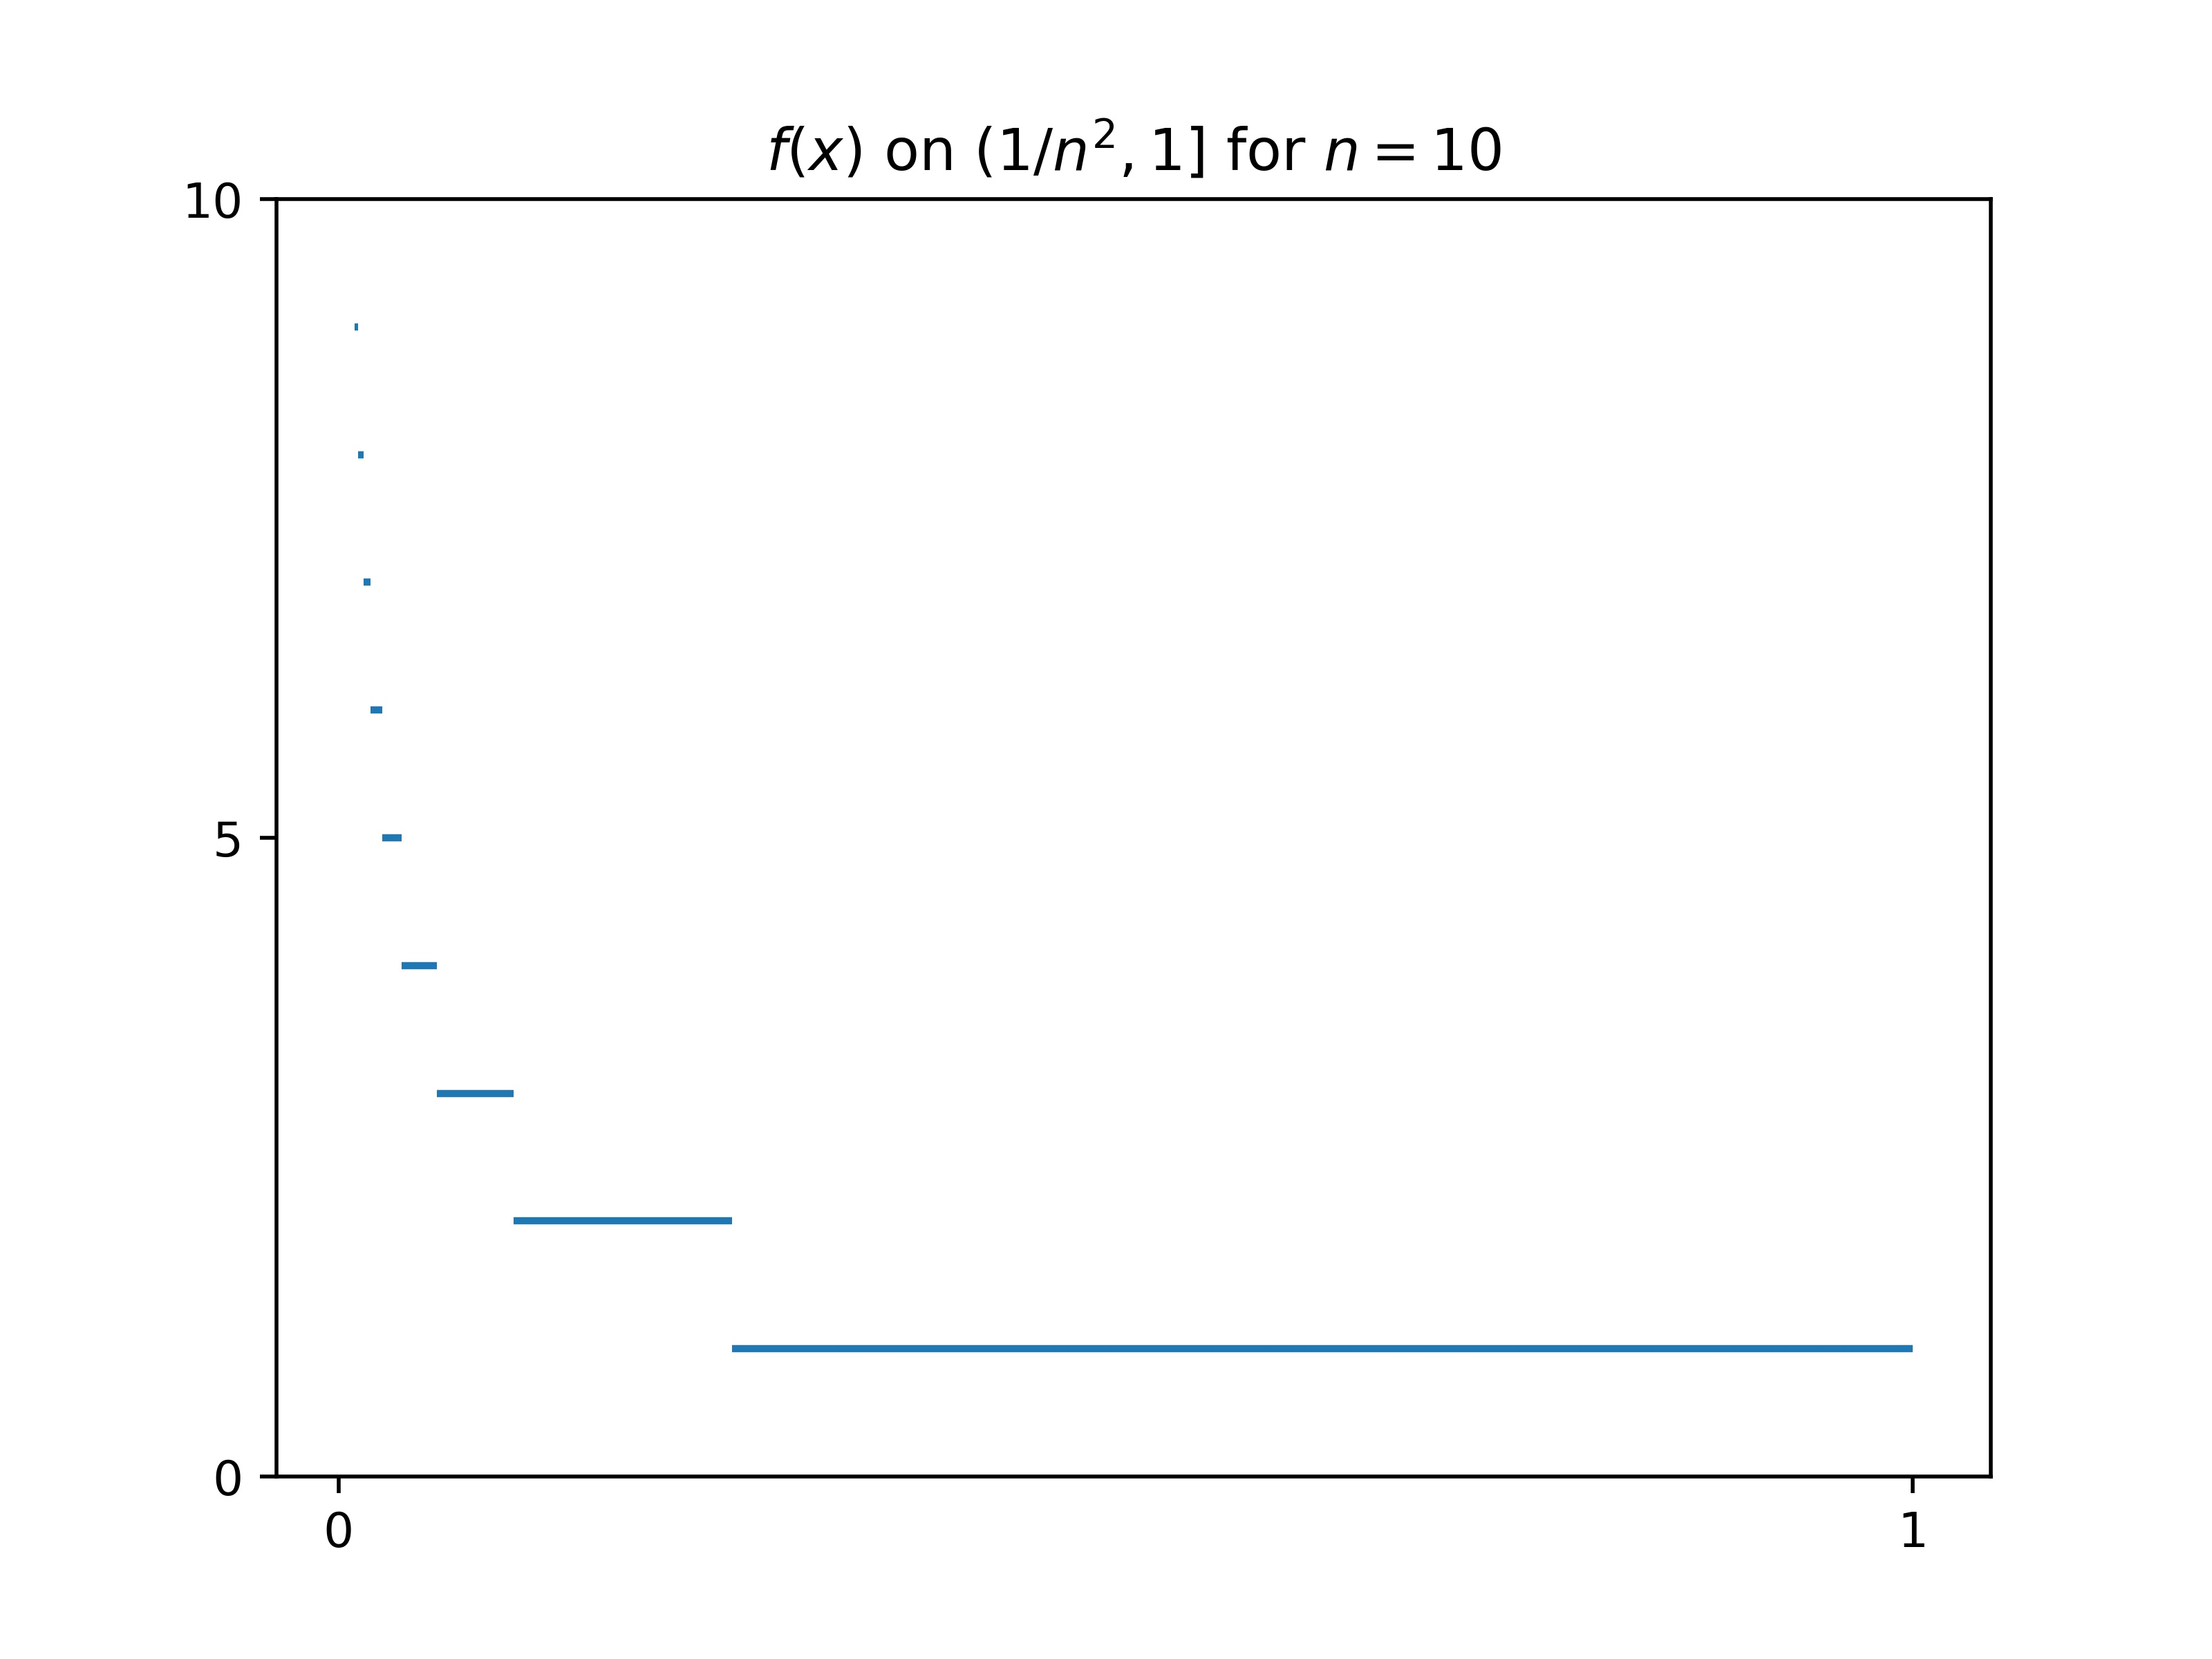
\includegraphics[width=15.5cm]{sketch.jpg}
\end{center}

\end{document}